% !TEX TS-program = pdflatex
\documentclass[final,3p,times]{elsarticle}
\usepackage{booktabs}
\usepackage{tabularx}
\usepackage{amsmath}
\usepackage{amssymb}
\usepackage{placeins}
\usepackage{float}
\usepackage{url}
\usepackage[hidelinks]{hyperref}
\usepackage{graphicx}
\usepackage{microtype}
\graphicspath{{figures/}}
\setlength{\textfloatsep}{10pt plus 2pt minus 2pt}
\setlength{\dbltextfloatsep}{10pt plus 2pt minus 2pt}
\bibliographystyle{elsarticle-num}
\journal{Computer Physics Communications}

\begin{document}
\begin{frontmatter}
\title{VARNEB: Calculator-agnostic variable-cell nudged elastic band calculations with auditable convergence acceleration and mode-resolved analysis}

% Draft metadata: confirm author order, affiliations, and contacts before submission.
\author[a]{Xudong Zhu}
\author[a]{VARNEB contributors}
\address[a]{Affiliation and postal address to be confirmed before submission}

\begin{abstract}
Solid--solid phase transitions require minimum-enthalpy paths in a space that
contains both atomic and cell degrees of freedom, yet most portable nudged
elastic band (NEB) workflows assume a common fixed cell or are tied to one
electronic-structure code. We present VARNEB, an open-source Python framework
for variable-cell NEB (VCNEB) calculations through an ASE-compatible
energy--force--stress contract. Each image is represented by fractional atomic
coordinates and a deformation gradient; atomic forces and stress are mapped to
one extended coordinate before tangent, spring, and climbing-image operations
are applied. A single manager owns the path, while isolated workers evaluate
only active interior images and fixed endpoints are cached. The same core is
used with ABACUS, VASP, Quantum ESPRESSO, CP2K, ABINIT, and generic ASE
calculators without backend branches in the path algorithm.

Finite-difference and fixed-cell reductions verify the generalized force
conventions. First-principles BaTiO$_3$ and HfO$_2$ paths validate image-count,
interpolation, climbing-image, and provenance controls. At 45.7 GPa, converged
29-image GaN B4-to-B1 calculations with ABACUS, VASP, Quantum ESPRESSO,
ABINIT, and CP2K give barriers of 0.3274, 0.3385, 0.3297, 0.2924, and
0.2928 eV/GaN,
respectively, and recover the same dominant barrier topology; the published
tetragonal-route value is 0.34 eV/GaN. A feasibility-aware family of
image-scaled, image-local, block, and staged FIRE updates reduces new image
evaluations by 38--79\% in controlled BTO/HfO$_2$ transfers, while preserving
negative transfer cases. Finally, a Phonopy-based $\Gamma$-mode projection
identifies the triply degenerate unstable cubic-BTO subspace as the principal
atomic component of the T-to-C path. VARNEB therefore contributes an
auditable, backend-independent execution and analysis layer around established
VCNEB theory, rather than claiming a new physical formalism.
\end{abstract}

\begin{keyword}
nudged elastic band \sep variable cell \sep crystal phase transition \sep
minimum-enthalpy path \sep calculator interoperability \sep phonon modes \sep
reproducible software
\end{keyword}
\end{frontmatter}

{\bf PROGRAM SUMMARY}
\begin{small}
\noindent {\em Program Title: VARNEB}\\
\noindent {\em CPC Library link to program files:} to be assigned under proof\\
\noindent {\em Developer's repository link:} \url{https://github.com/xdzhu/varneb}\\
\noindent {\em Licensing provisions: GNU General Public License 3.0 or later}\\
\noindent {\em Programming language: Python}\\
\noindent {\em Nature of problem:} Conventional NEB implementations commonly
assume a shared simulation cell. Solid--solid transitions may change cell
lengths, angles, and volume, and require atomic and cell forces to be treated
in a common path metric. Robust production workflows must also retain endpoint
mapping, calculator settings, scheduler resources, restart state, and
image-level evidence.\\
\noindent {\em Solution method:} VARNEB represents each image by fractional
atomic coordinates and a reference-cell deformation gradient. Cartesian forces
and stress are transformed into generalized forces before the improved tangent,
spring, and climbing-image projections are evaluated. Calculator adapters
return energy, force, and stress through ASE-compatible interfaces. The
optimizer and calculator are independent choices. A single manager owns the
path while isolated workers evaluate interior images concurrently; fixed
endpoints are evaluated once. Image-local and staged step control is combined
with a pre-calculation cell-feasibility gate. JSON summaries, trajectories,
audits, source-data exports, and mode projections provide reproducible reports.
\end{small}

\section{Introduction}
\label{sec:introduction}

Solid--solid phase transitions couple collective atomic motion to changes in
the lattice. This makes a fixed-cell reaction coordinate insufficient when the
minimum-enthalpy path changes volume, shape, or shear. Variable-cell NEB was
formulated for such transitions by Qian \emph{et al.}\ \cite{Qian2013}; related
generalized solid-state NEB (G-SSNEB) and finite-deformation approaches clarify
the role of cell metrics, external loading, and work-conjugate stress measures
\cite{Sheppard2012,Ghasemi2019}. These developments establish the physical
method. They do not, by themselves, supply a portable implementation in which
the same path controller can be tested with multiple electronic-structure
codes, interrupted safely on a scheduler, or interrogated in a vibrational
mode basis.

ASE provides a widely used calculator abstraction and fixed-cell NEB tools
\cite{Larsen2017}, but its NEB object does not optimize periodic images with
different cells. Production first-principles calculations also require more
than an optimizer loop. Every image needs an isolated calculator directory;
static calculator settings must not be confused with ionic relaxation; the
path controller must prevent endpoint recomputation and worker races; and
force, stress, image-count, and restart diagnostics must remain auditable.
These requirements become especially important when one compares plane-wave,
localized-orbital, Gaussian/plane-wave, and pseudopotential implementations.

VARNEB addresses these requirements as a pure-Python package. It treats VASP
\cite{Kresse1996a,Kresse1996b}, ABACUS \cite{Li2016}, Quantum ESPRESSO
\cite{Giannozzi2017}, CP2K \cite{Kuhne2020}, ABINIT \cite{Gonze2020}, and
generic ASE calculators as external providers of energy, Cartesian forces,
and stress. The physical path formulation follows established VCNEB work;
VARNEB's software contributions are three linked capabilities. First, one
manager--worker implementation executes the same variable-cell path with
independent calculators while preserving endpoint identity and a restartable
record. Second, image-local and staged updates combine with a pre-calculation
feasibility gate to reduce expensive image evaluations; matched starting
chains and negative transfers bound the speed claim. Third, endpoint phonon
eigenvectors resolve the atomic part of a converged path into invariant mode
subspaces while cell strain remains explicit. We test these claims with a
barrierless BTO path, an activated HfO$_2$ path, five completed GaN backends,
and mapping-sensitive controls. Material-level agreement requires a recorded
pressure, normalization, endpoint identity, calculator contract, complete
force/stress record, and convergence audit.

\section{From conventional NEB to VCNEB}
\label{sec:method}

\subsection{Conventional fixed-cell NEB}

For a fixed simulation cell, an image is represented only by its Cartesian
coordinate vector $R_i\in\mathbb{R}^{3N}$.  NEB finds a discretized
minimum-energy path by retaining the physical force perpendicular to the local
path tangent $\hat\tau_i$ and adding a spring force parallel to it.  With
$d_i^{\pm}=\lVert R_{i\pm1}-R_i\rVert$, the standard interior-image force is
\begin{equation}
 f_i^{\mathrm{NEB}}=
 f_i-(f_i\cdot\hat\tau_i)\hat\tau_i+
 k_i(d_i^+-d_i^-)\hat\tau_i .
 \label{eq:fixed-neb}
\end{equation}
This separation prevents the true force from sliding images down the path while
the springs control their spacing.  A climbing image replaces this expression
only after an ordinary band has formed an interior energy maximum: it reverses
the tangent component of the true force and removes the spring
\cite{Henkelman2000}.  Fixed-cell NEB is therefore recovered whenever every
image shares the same $h$ and cell degrees of freedom are inactive.

\subsection{Variable-cell generalized coordinates}

For an image with $N$ atoms, let $h$ be the row-vector cell matrix, $s_a$ the
fractional coordinate of atom $a$, and $h_0$ a reference cell. VARNEB writes
\begin{equation}
 r_a=s_a h,\qquad h=h_0F^T,
\end{equation}
where $F$ is a deformation gradient. The optimizer coordinate is
\begin{equation}
 x(Q)=\left(\operatorname{vec}(s h_0),c\operatorname{vec}(F-I)\right),
 \label{eq:coordinate}
\end{equation}
with $c$ a user-visible cell scale. Thus $c$ is a numerical metric choice, not
a material constant, and is recorded in summaries and sensitivity checks.

At hydrostatic pressure $P$, the target is $H(Q)=E(Q)+P\Omega(Q)$. For
calculator stress $\sigma$, the row-vector convention gives the cell
contribution through
\begin{equation}
 W=-\Omega(\sigma+PI),\qquad g_F=WF^{-T}.
 \label{eq:cellforce}
\end{equation}
The atomic and cell blocks are transformed into the common coordinate in
Eq.~\ref{eq:coordinate} before tangential projection.  Thus the fixed-cell
construction in Eq.~\ref{eq:fixed-neb} carries over without assigning
independent, incompatible reaction coordinates to atoms and the lattice.  For
internal image $i$, the ordinary generalized path force is
\begin{equation}
 g_i^{\mathrm{NEB}}=g_i-(g_i\cdot\tau_i)\tau_i+
 k_i(d_i^+-d_i^-)\tau_i.
 \label{eq:nebforce}
\end{equation}
The climbing-image replacement reverses the tangential component of the true
generalized force and removes the spring. CI is enabled only after an ordinary
path has a real interior enthalpy peak above both endpoints. A negative local
tangent curvature alone is not enough: a monotonic band can otherwise produce
a formal highest internal image that is not a transition state
\cite{Henkelman2000}.

Endpoint mapping and periodic translation gauge are validated before an
expensive run. The path preflight records minimum periodic atom separation,
cell deformation, segment length, and folded junctions. Summaries retain the
maximum generalized force, atom-force and stress components, reaction enthalpy,
barrier, peak identity, and CI status. An explicit post-run loose NEB re-audit
never changes the trajectory or its calculator settings.

\subsection{Mode-resolved path coordinates}
\label{sec:modes}

The path itself is a sequence of generalized coordinates, but its atomic part
can be interpreted in a vibrational basis after a calculation. Let
$e_\nu$ be mass-normalized $\Gamma$-point eigenvectors of a selected endpoint,
$M$ the diagonal atomic-mass matrix, and $u_i$ the Cartesian displacement of
image $i$ after applying the recorded atom mapping, periodic translation
gauge, and rigid-translation removal. VARNEB evaluates
\begin{equation}
 q_{i\nu}=e_\nu^{T}M^{1/2}u_i .
 \label{eq:mode-coordinate}
\end{equation}
Because eigenvectors inside an exactly or nearly degenerate manifold are not
unique, the invariant reported quantity is the subspace norm
\begin{equation}
 Q_{i\mathcal{S}}=\left(\sum_{\nu\in\mathcal{S}}q_{i\nu}^{2}\right)^{1/2},
 \label{eq:subspace-coordinate}
\end{equation}
rather than the amplitude of one arbitrarily phased vector. Segment-tangent
overlaps identify which subspaces drive local path evolution, and complete
basis reconstruction provides a numerical check. Homogeneous strain is kept
as a separate VCNEB coordinate; it is not relabelled as a phonon amplitude.
The same mode objects can guide an initial path or define a temporary strict
subspace, but any constrained result intended as a physical path is released
and reconverged in the full generalized space.

\subsection{Convergence-aware path optimization}
\label{sec:acceleration}

The extended coordinate couples displacement blocks with different numerical
scales. In addition, a global FIRE step cap is shared by all active images, so
its effective per-image displacement decreases approximately as
$N_{\mathrm{int}}^{-1/2}$ when the number of interior images is increased.
VARNEB therefore exposes three related controls. ImageScaledFIRE interprets a
user step cap as a per-interior-image scale and applies the corresponding
$\sqrt{N_{\mathrm{int}}}$ correction. BlockFIRE gives each image an independent
FIRE state, time step, and displacement cap; SplitFIRE further separates the
atomic and cell blocks. StagedFIRE begins with the image-normalized cap and
switches to a smaller cap after a force threshold, resetting momentum at the
switch. All variants retain the FIRE update logic \cite{Bitzek2006}. These
controls are separated from the physical path metric: they
change the update sequence while leaving the energy, force, stress, tangent,
and spring definitions unchanged. Related ideas exist for fixed-cell NEB and
preconditioned path optimization \cite{Makri2019,Kolsbjerg2016,Lindgren2019};
our implementation targets their variable-cell, calculator-backed execution
failure modes.

The feasibility gate sits between the optimizer and the
calculator. Before a candidate image is sent to DFT, VARNEB checks positive
cell volume, conditioning, minimum periodic separation, serialized-cell round
trip, and an optional calculator-native lattice probe. A rejected candidate is
shortened only for the affected image and its local optimizer state is reset.
An electronic failure is treated separately: the identical input may be
retried within a finite budget, but physical parameters are not changed. This
makes recovery auditable and prevents a bad cell proposal from being silently
converted into a different calculation. Section~\ref{sec:efficiency} tests the
effect of these controls with matched first-principles starting chains.

\section{Calculator-agnostic architecture and reproducible workflow}
\label{sec:software}

The core receives no program-specific input keywords. Its calculator contract
requires finite energy, Cartesian forces, and stress for every image; missing
stress is a hard failure because the cell generalized force would be undefined.
A backend factory owns units, stress convention, pseudopotential and basis
metadata, static single-point semantics, launch command, and a unique working
directory. The external calculator must not perform an ionic or cell
relaxation inside an image: the VARNEB manager is the sole owner of $Q_i$
updates. Consequently, the backend and optimizer are orthogonal choices. The
same VCNEB object can use a conservative BlockFIRE update with VASP or ABACUS,
for example, without a backend branch in the tangent or force code.

\begin{figure}[H]
\centering
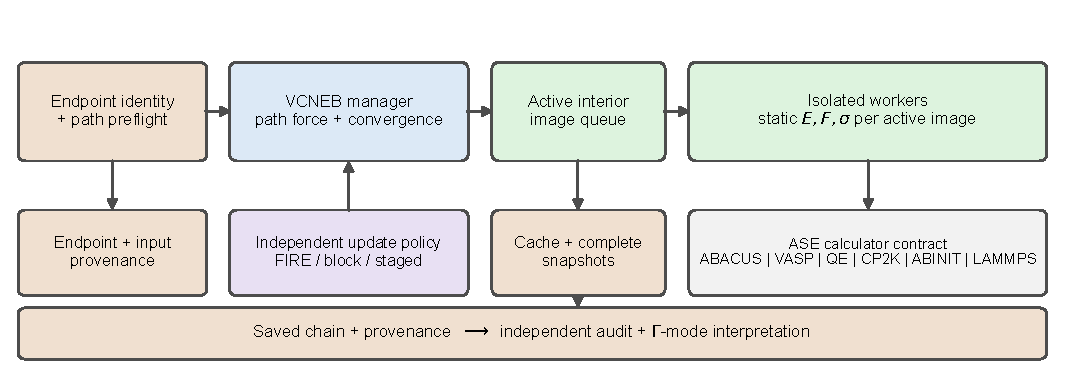
\includegraphics[width=\textwidth]{figures/varneb_architecture.pdf}
\caption{VARNEB software architecture. Endpoint identity, mapping, and path
geometry are checked before DFT. One calculator-independent manager owns image
order, the path force, optimizer state, convergence, and restart data. Only
active interior images are sent to isolated workers, each of which returns a
static energy, force, and stress tuple through an ASE-compatible adapter;
fixed endpoints are cached once. The update policy is independent of the
calculator choice. Audits and mode
projections consume the same durable trajectory and provenance records.}
\label{fig:architecture}
\end{figure}

Specialized factories cover the file and process protocols of ABACUS, VASP,
Quantum ESPRESSO, CP2K, and ABINIT; a generic factory accepts any ASE calculator
that supplies the required properties. Each image has a private calculator
directory, so no worker shares mutable restart, scratch, or output files. A
threaded executor delegates only static calculator calls. Endpoints are fixed
and cached, so a 7-total-image calculation has five costly interior images,
not seven repeated endpoint evaluations. Figure~\ref{fig:architecture}
summarizes this ownership model.

Each calculator-free preflight records an ordered endpoint identity from
species, periodicity, cell, and wrapped fractional coordinates. A production
gate then requires the effective mapped endpoints to match the independently
accepted static references. This distinction caught a CP2K case in which a
translation alignment changed the real-space-grid representation of the
effective final endpoint: the source structure had passed, but the structure
actually used by the path had not. The repaired workflow gates the effective
hash and therefore prevents an atom reorder or coordinate-gauge change from
being misreported as a backend comparison of the same path.

The durable image cache is keyed by exact configuration plus calculator
namespace. If a batch partially fails, completed sibling evaluations remain
available and the manager emits a structured failure report. Restart selects a
complete chain snapshot; it does not regenerate an interpolation or overwrite
the original initial chain.

Backend independence also requires a numerical serialization contract. The
VASP adapter freezes the static parameters and licensed-input fingerprints,
then writes lattice components with 17 significant decimal digits and verifies
exact binary64 round-trip before launching the executable.  The optional
lattice preflight evaluates the same serialized cell, so a last-digit POSCAR
rounding change cannot silently alter VASP's direct/reciprocal Bravais
classification.  This check does not symmetrize an image or adjust
\texttt{SYMPREC}; a diagnostic linked to a local licensed VASP object must be
validated against the corresponding executable and compiler target.  Its
failure rejects the complete candidate before any image worker is launched.
QE is restricted to static \texttt{scf} evaluations, ABINIT uses an explicit
pseudopotential manifest, and the CP2K shell is created lazily for one image
evaluation and closed afterwards. These rules are backend details, but their
observable contract at the controller boundary remains the same $(E,F,\sigma)$
tuple.

\begin{table*}[t]
\centering
\caption{Current VARNEB capabilities and evidence boundaries.}
\label{tab:capabilities}
\begin{tabularx}{\textwidth}{>{\raggedright\arraybackslash}p{0.22\textwidth}>{\raggedright\arraybackslash}X>{\raggedright\arraybackslash}p{0.28\textwidth}}
\toprule
Capability & Delivered behaviour & Evidence boundary \\
\midrule
Extended VC-NEB coordinate & Fractional atom coordinates, deformation gradient,
force/stress transformation, pressure and cell masks & Analytic finite differences
and fixed-cell reduction tests \\
Path search & Ordinary NEB, staged CI, FIRE/BFGS/LBFGS interfaces, linear or
log-strain cell interpolation & CI requires an interior-barrier gate \\
Mode APIs & Initial-path guidance, strict subspace and projected-update modes,
endpoint $\Gamma$ eigenvectors, degenerate-subspace coordinates, and tangent
overlaps & BTO endpoint force constants and a seven-image path projection are
archived; strict real-material release-and-refine remains incomplete \\
Execution & Isolated image directories, manager/worker ownership, bounded retry,
snapshots, resume and durable cache & Scheduler resources remain user-reviewed \\
Calculators & ABACUS, VASP, QE, CP2K, ABINIT, LAMMPS, and a generic ASE
factory & Material-level evidence is reported separately from adapter-level
availability; LAMMPS remains potential-dependent \\
Reporting & JSON summary, trajectory, audit, image comparison, structural metrics,
source-data and editable figure export & Results remain calculator and
boundary-condition specific \\
\bottomrule
\end{tabularx}
\end{table*}

A production run prepares element-preserving endpoint structures with identical
atom count, independently relaxes and audits them, preflights a mapped and
translation-aligned initial path, runs ordinary VC-NEB with cached endpoints,
compares image counts, and only then enables CI. The command-line driver
exposes image count, cell interpolation, mapping, force threshold, image
workers, and resume state rather than choosing them implicitly. Complete,
backend-specific invocations are maintained with the executable examples so
that the manuscript is not a second, divergent user manual.

\section{Validation and material examples}
\label{sec:results}

An analytic coupled atomic--cell multiwell potential supplies a known minimum,
saddle, and 0.25 eV barrier. Finite-difference tests cover atomic forces, cell
forces, nonzero pressure, and nonorthogonal cells. A fixed-cell comparison with
ASE NEB/CINEB gives a barrier difference of $9.33\times10^{-6}$ eV under the
matched test convention. These tests establish implementation consistency, not
first-principles predictive accuracy.

\subsection{Numerical protocol and evidence levels}

All production paths use independently relaxed endpoints, fixed endpoints
during band optimization, and a maximum generalized-force target of
$0.10$ eV/\AA{}. ``Total images'' always includes the two endpoints. A path is
accepted only when every image has finite energy, force, and stress; the path
geometry audit passes; and the recorded threshold is met. Endpoint relaxation
uses separate atomic-force and pressure-residual tests, because a small atomic
force alone does not establish a relaxed cell. Climbing-image refinement is
allowed only after an ordinary path contains a genuine interior maximum.

Table~\ref{tab:calculators} records the principal first-principles contracts.
The rows are intentionally not forced to share a basis or pseudopotential
formalism. Cross-backend comparison tests whether the same controller can
recover a consistent path topology and barrier scale under independently
converged calculator contracts; it is not a subtraction of total energies from
different codes. QE and ABINIT use the PseudoDojo norm-conserving PBE family
\cite{vanSetten2018}. CP2K uses a mixed Gaussian/plane-wave representation,
whereas VASP and QE use plane waves and ABACUS uses numerical atomic orbitals.

\begin{table*}[t]
\centering
\caption{Principal material-level calculator contracts used in this work.
The GaN runs have 29 total images (27 interior) at 45.7 GPa. Every GaN row
corresponds to a completed path satisfying the common 0.10 eV/\AA{} force
criterion, with finite image energy, force, and stress.}
\label{tab:calculators}
\begin{tabularx}{\textwidth}{l l l l l >{\raggedright\arraybackslash}X}
\toprule
Backend & XC & Basis/potential & Cutoff & $k$ mesh & Material evidence \\
\midrule
ABACUS & PBE & Dojo NC, 10-au DZP & 100 Ry & $4\times4\times3$ & GaN complete; BTO/HfO$_2$ complete \\
VASP 6.3.2 & PBE & Ga$_d$/N PAW & 600 eV & $8\times8\times6$ & GaN complete; additional BTO/HfO$_2$/CdSe paths \\
QE 7.0 & PBE & PseudoDojo NC-SR UPF & 100/600 Ry & $4\times4\times3$ & GaN complete \\
ABINIT 8.6.1 & PBE & PseudoDojo NC-SR PSP8 & 1400 eV & $4\times4\times3$ & GaN complete \\
CP2K 2024.1 & PBE & GTH-PBE/DZVP-MOLOPT-SR & 800/80 Ry & $4\times4\times3$ & GaN and BTO paths complete \\
\bottomrule
\end{tabularx}
\end{table*}

\subsection{BaTiO$_3$ tetragonal to cubic path}

BaTiO$_3$ is a compact direct perovskite case. ABACUS/PBE calculations use
100 Ry and full 10-au DZP Ba/Ti/O orbitals, a $4\times4\times4$ k mesh, and
independently relaxed fixed endpoints. Ordinary 5-, 7-, and 9-total-image paths
meet the default $0.10$ eV/\AA{} maximum-generalized-force criterion and are
all monotonic.
Their reaction enthalpy is $0.0871289$ eV per formula unit; there is no interior
barrier, so CI is correctly withheld. A tighter $6\times6\times6$ and $10^{-9}$
SCF comparison preserves the path topology but shifts the absolute endpoint
difference by about 15 meV. An independent CP2K/PBE calculation with nine
total images also converges without an interior maximum
($f_{\max}=0.08183$ eV/\AA{}); its endpoint rise is 0.06080 eV/f.u. The CP2K
run is a topology and calculator-contract check, not a demand that the standard
BTO workflow use nine images: seven total images (five interior) remains the
compact production choice.

The result corresponds to $2.01$ kcal mol$^{-1}$ and is close in energy scale
to a reported $2.1$ kcal mol$^{-1}$ restrained PBEsol NEB result
\cite{BTOReaxFF2019}. This is not a strict algorithm benchmark: the literature
calculation uses different exchange-correlation treatment and local restraints,
whereas the present result is an unconstrained variable-cell path.

To separate a path-coordinate description from a phonon claim, we also evaluated
the cubic endpoint with a $1\times1\times1$ finite-displacement calculation
($\delta=0.01$ \AA{}, six signed displacements) and assembled the $\Gamma$-point
force constants and direct $\Gamma$ eigenvectors with Phonopy \cite{Togo2015}.
The ABACUS--Phonopy force-constant convention,
$\mathrm{eV}/(\text{\AA}\,\mathrm{au})$, is retained explicitly in the provenance
of the direct Phonopy $q=0$ calculation. The spectrum contains a triply degenerate unstable
subspace at $-298.956$ cm$^{-1}$. After applying the
recorded O-atom permutation and endpoint translation gauge, then removing each
image's mass-weighted rigid translation, the seven-image T-to-C atomic path has
a maximum soft-subspace coordinate norm of $1.2043\sqrt{\mathrm{amu}}$\AA{} and
a maximum segment-tangent overlap of 0.9974 with that subspace. The complete-mode
reconstruction residual is below $5.9\times10^{-16}\sqrt{\mathrm{amu}}$\AA{}.
The $175.809$ cm$^{-1}$ stable triplet also participates (maximum coordinate norm
$0.2863\sqrt{\mathrm{amu}}$\AA{}), so this is a subspace-resolved mechanism
analysis rather than an assertion that one arbitrarily phased eigenvector alone
defines the path. Homogeneous cell strain remains a separate VC-NEB coordinate,
not a phonon amplitude.

\begin{figure*}[t]
\centering

\includegraphics[width=\textwidth]{figures/bto_gamma_mode_path.pdf}
\caption{BTO T-to-C path resolved in cubic-endpoint $\Gamma$ subspaces. (a)
Mass-weighted coordinate norms after applying the recorded atom permutation and
endpoint gauge translation, then removing each image's rigid translation. The
threefold unstable subspace (purple) dominates the atomic path; stable triplets
are retained to show the residual multimode component. (b) The same seven-image
ABACUS/PBE path has no interior energy maximum. (c) Homogeneous volume evolution
is reported separately from the atomic phonon coordinates. This is one
deterministic first-principles path, so no statistical error bars are implied.
Editable source data accompany the manuscript.}
\label{fig:bto-gamma-mode}
\end{figure*}

\subsection{HfO$_2$ tetragonal to polar orthorhombic path}

The HfO$_2$ case uses an explicitly mapped 12-atom Hf$_4$O$_8$ endpoint pair:
a $\sqrt{2}\times\sqrt{2}\times1$ tetragonal supercell and a
conventional-compatible polar orthorhombic cell. ABACUS/PBE calculations use
100 Ry, full 10-au DZP Hf/O orbitals, a $2\times2\times2$ k mesh, and
independently converged endpoints. Ordinary log-strain 7- and 9-total-image
paths give barriers of 0.1567509 and 0.1562092 eV per 12-atom cell,
respectively, a spread of 0.0005417 eV. The 7-image linear-cell control is
0.1596772 eV. These controls are reported separately: the linear-cell path
tests interpolation sensitivity rather than image-count convergence.

The staged 7-image CI refinement gives 0.1291722 eV per 12-atom cell, or
32.29 meV per HfO$_2$ formula unit, at a final maximum generalized force of
0.02955 eV/\AA{}. Liu and Hanrahan reported 32 meV per formula unit for a
40-image LDA/QE/USPEX VC-NEB calculation \cite{Liu2019}. The agreement is
encouraging but deliberately qualified by functional, pseudopotential,
implementation, image-count, mapping, and force-norm differences.

A separate real-material release diagnostic starts from a strict-subspace
chain and then releases all degrees of freedom.  Its full-space force reached
0.097528 eV/\AA{} at step 275 but rebounded to 0.108376 eV/\AA{} during 25
additional observed steps.  We archive the step-275 path only under the
conventional loose 0.10 eV/\AA{} ordinary-NEB convention; it is excluded from
the strict ordinary/CI barrier comparison and literature discussion.

\begin{figure*}[!t]
\centering

\includegraphics[width=0.96\textwidth]{figures/vcneb_material_validation.pdf}
\caption{Material validation and qualified literature comparison. (a) ABACUS/PBE
BaTiO$_3$ T-to-C paths at 5, 7, and 9 total images are monotonic; the cubic
endpoint rise is 0.08713 eV/f.u. and no internal image is a maximum. (b)
HfO$_2$ T-to-PO ordinary
log-strain paths, a linear-cell control, and a staged CI refinement. The open
circle marks the climbing image and the dotted line denotes the external
literature CI-VCNEB barrier. (c) HfO$_2$ barriers per formula unit. The
literature bar is not a statistical replicate. (d) Relative volume evolution
demonstrates the variable-cell degree of freedom. Source data accompany this
figure in the software archive.}
\label{fig:materials}
\end{figure*}

\subsection{Calculator-work reduction on matched chains}
\label{sec:efficiency}

Table~\ref{tab:acceleration} isolates the update policy from the calculator:
each comparison starts from the same archived chain and holds the endpoints,
image count, spring, pressure, calculator settings, and $0.10$ eV/\AA{}
stopping rule fixed. New image evaluations are counted from manager logs; wall
time is reported for context but includes scheduler and filesystem variation.
All listed variants reach the common force threshold and retain the same
endpoint-defined energy scale.

\begin{table}[H]
\centering
\footnotesize
\caption{First-principles convergence ablations. $n$ denotes total images;
``saved'' compares new image evaluations with global FIRE for the same case.
The final generalized force is in eV/\AA{}.}
\label{tab:acceleration}
\begin{tabular}{@{}llrrrrr@{}}
\toprule
Case & Update policy & Steps & Time (s) & New image evals & Saved (\%) & Final $f_{\max}$ \\
\midrule
BTO $n=9$ & global FIRE & 28 & 2669 & 205 & --- & 0.0967 \\
BTO $n=9$ & BlockFIRE (0.02/image) & 10 & 963 & 79 & 61.5 & 0.0865 \\
BTO $n=9$ & BlockFIRE (0.01/image) & 5 & 478 & 44 & 78.5 & 0.0899 \\
BTO $n=9$ & ImageScaledFIRE & 8 & 772 & 65 & 68.3 & 0.0781 \\
HfO$_2$ $n=7$ & global FIRE & 42 & 5242 & 217 & --- & 0.0942 \\
HfO$_2$ $n=7$ & StagedFIRE & 24 & 3513 & 134 & 38.2 & 0.0924 \\
\bottomrule
\end{tabular}
\end{table}

The conservative BTO BlockFIRE setting lowers new image evaluations by
78.5\% and measured threshold time by 82.1\%; the staged HfO$_2$ transfer
lowers them by 38.2\% and 33.0\%, respectively. A matched global-cap control
and a SplitFIRE transfer in the project benchmark show negative transfer, and
BlockFIRE plateaus on one 20-image HfO$_2$ chain. These observations support
the image-local and staged controls on the tested chains, while leaving the
best update policy material- and path-dependent.

\subsection{GaN B4-to-B1 across first-principles backends}
\label{sec:gan-multibackend}

GaN B4-to-B1 at 45.7 GPa supplies a finite-barrier production benchmark. The
four-atom path contains 29 total images, uses the tetragonal mapping of the
Qian benchmark, and normalizes enthalpy by two GaN formula units. Nine image
workers evaluate the 27 interior images in three waves for ABACUS, QE, and
ABINIT; VASP uses the same manager ownership and endpoint-cache policy. The
launcher within a worker is backend-specific and is recorded rather than
inferred: four MPI ranks for ABACUS, 32 for VASP, one exclusive Slurm rank for
QE, eight Hydra ranks for ABINIT, and 16 MPI ranks in each of five CP2K
workers. The latter evaluates the 27 interior images in six waves.

All five completed calculations meet $f_{\max}\leq0.10$ eV/\AA{} and place
the dominant maximum at image 15 (Fig.~\ref{fig:gan-multibackend}). Their
barriers are 0.3274, 0.3385, 0.3297, 0.2924, and 0.2928 eV/GaN for ABACUS,
VASP, QE, ABINIT, and CP2K, respectively. The first three lie within
0.013 eV/GaN of the
0.34 eV/GaN tetragonal-route value reported by Qian \emph{et al.}
\cite{Qian2013}; ABINIT and CP2K are lower by 0.0476 and 0.0472 eV/GaN.
The endpoint reaction
enthalpy is more code-sensitive ($-0.0585$ to $-0.0046$ eV/GaN), as expected
for independently relaxed endpoint geometries and distinct basis and
pseudopotential families. The defensible cross-backend claim is therefore a
common dominant topology and barrier scale, not numerical identity.

\begin{figure*}[t]
\centering
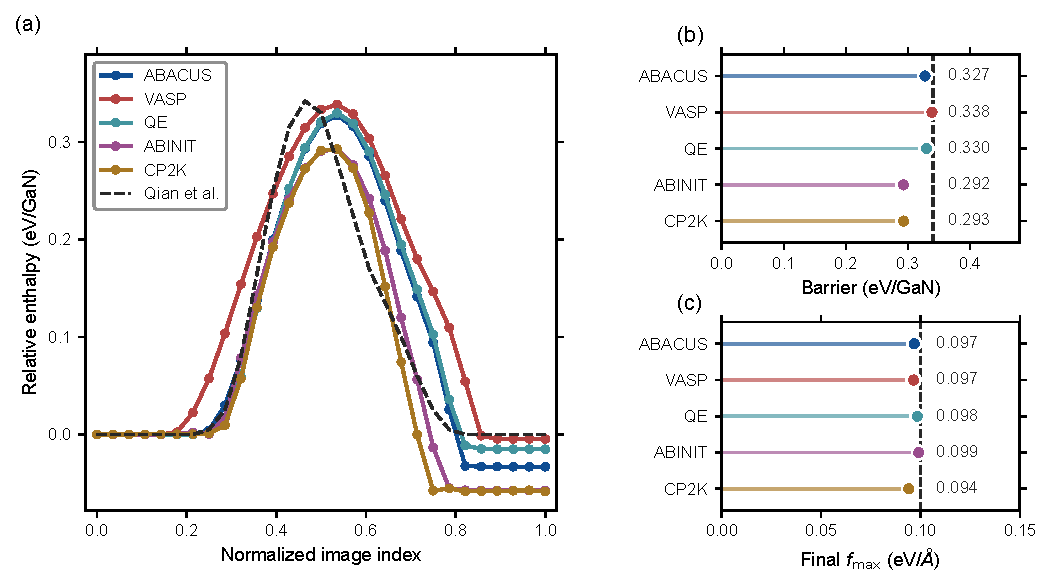
\includegraphics[width=\textwidth]{figures/gan_multibackend_validation.pdf}
\caption{Multi-backend GaN B4-to-B1 benchmark at 45.7 GPa. (a) Converged
29-total-image ordinary VCNEB enthalpy paths plotted against image index divided
by 28. The dashed literature curve is an approximate digitization of the
tetragonal route in Ref.~\cite{Qian2013}; each curve is referenced to its own
initial endpoint, and the shape comparison is qualitative. (b) Barrier
comparison with the published 0.34 eV/GaN value (vertical dashed line). (c)
Final maximum generalized force and the common 0.10 eV/\AA{} threshold
(vertical dashed line). All five backend paths are converged and include
the complete CP2K chain rather than an endpoint-only or provisional result.}
\label{fig:gan-multibackend}
\end{figure*}

The CP2K path uses the same pressure, phases, atom order, image count, and
controller settings. Its endpoint pressure residuals are 0.416 and 0.249 kbar,
both below the 1 kbar gate. The ordinary-NEB path reaches
$f_{\max}=0.09409$ eV/\AA{} after 52 updates; all 29 images have finite
energy, force, and stress, the saved-band endpoint hashes match the static
references, and the geometry audit passes. The 0.29276 eV/GaN barrier is
located at image 15. These checks distinguish the complete path result from
an endpoint-only backend demonstration.

\subsection{Additional path-transfer benchmarks}

VASP 6.3.2/PBE additionally exercises long-path restart, lattice
serialization, candidate feasibility, and mapping sensitivity. Endpoints are
not dispatched during each iteration; static PAW data, $k$ points,
$\mathrm{ISYM}=-1$, and $\mathrm{SYMPREC}=10^{-4}$ remain fixed. Table~\ref{tab:vasp}
lists the additional completed paths. GaN energies are divided by the number
of formula units in the conventional cell. CdSe is reported in meV/atom
because the published G-SSNEB landscape has a small barrier.

\begin{table}[!htbp]
\centering
\footnotesize
\caption{Additional completed VASP paths not included in the GaN
multi-backend panel. The literature values are comparison
references with their own functionals, coordinate metrics, and image protocols;
they are not treated as exact cross-code replicas.}
\label{tab:vasp}
\begin{tabularx}{\textwidth}{p{0.25\textwidth}l c c c >{\raggedright\arraybackslash}X}
\toprule
Path & Pressure & $N_{\mathrm{total}}$ ($N_{\mathrm{int}}$) & VARNEB barrier & Literature & Interpretation \\
\midrule
GaN B4$\rightarrow$B1, hexagonal & 45.7 GPa & 29 (27) & 0.3852 eV/GaN & 0.39 eV/GaN & barrier agrees; digitized shape agrees \\
GaN B3$\rightarrow$B1 & 45.0 GPa & 29 (27) & 0.9553 eV/GaN & $\simeq$0.57 eV/GaN & mapping-sensitive negative control \\
CdSe RS$\rightarrow$WZ, cell mapping & 0 GPa & 17 (15) & 7.22 meV/atom & 2.4 meV/atom & PBE/PW91 and metric differ \\
HfO$_2$ T$\rightarrow$PO & 0 GPa & 20 (18) & 2.97 meV/f.u. & 2.50 meV/f.u. & same downhill topology \\
HfO$_2$ PO$\rightarrow$M & 0 GPa & 20 (18) & 83.6 meV/f.u. & 105.1 meV/f.u. & same single-barrier topology \\
\bottomrule
\end{tabularx}
\end{table}

The tetragonal and hexagonal GaN routes are within 0.002 and 0.005 eV/GaN of
their respective Qian \emph{et al.} values \cite{Qian2013}. The
B3$\rightarrow$B1 negative control is scientifically useful because the
present diagonal mapping produces one broad high barrier, whereas the
reference chain contains three connected events. Those events must be treated
as three joined path segments if one wants separate elementary barriers; a
single long-chain three-peak trace is not evidence for three independently
converged calculations. The discrepancy is therefore assigned to path
construction, not to the VASP adapter.
For CdSe, the current PBE result is compared with the PW91 G-SSNEB landscape
of Sheppard et al. \cite{Sheppard2012}; the small barrier and different
coordinate definition preclude a claim of quantitative reproduction. The full
per-path figures, digitization flags, hashes, and CSV source data are archived
under \texttt{outputs/neb\_literature\_benchmarks/}.

\FloatBarrier
\section{Scope, limitations, and outlook}
\label{sec:limits}

VARNEB currently implements the documented hydrostatic enthalpy convention.
General-stress G-SSNEB and finite-deformation paths require an explicit choice
of strain coordinate and work-conjugate stress; they are not silently inferred
from the hydrostatic interface. Likewise, a converged climbing image is not by
itself a vibrational proof of a first-order saddle. Targeted Hessian analysis
is still required when that designation is scientifically essential.

The cross-backend GaN result establishes interoperability and a stable barrier
scale, not universal DFT accuracy. Endpoint relaxation, pseudopotentials,
basis completeness, Brillouin-zone sampling, and stress implementations remain
part of each calculator's uncertainty. HfO$_2$ remains sensitive to mapping,
supercell size, mechanical boundary conditions, and possible intermediate
mechanisms. The BTO case is deliberately barrierless and validates the CI gate
rather than a saddle search. The CP2K GaN result now passes the same path
threshold and full-image audit as the other production backends; its lower
barrier does not establish which code is closer to the exact functional limit.

The acceleration evidence is also bounded. Image-local state is highly
effective for the BTO ablation and rescues CdSe and selected VASP chains, but
it plateaus on one 20-image HfO$_2$ transfer. The supported contribution is the
combination of image-count normalization, local state isolation, staged trust
radii, and pre-DFT feasibility checks with explicit failure semantics. Future
work will test a metric-consistent atom--strain preconditioner, adaptive image
insertion followed by a frozen-image recertification, and strict
release-and-refine mode-guided paths.

\section{Conclusions}

VARNEB makes established VCNEB physics usable through a documented generalized
force, calculator, execution, and evidence contract. Five converged GaN
backends share one 29-image path controller and recover the same dominant
barrier topology. On matched BTO and HfO$_2$ chains, image-local or staged updates
reduce new calculator evaluations by 78.5\% and 38.2\%, respectively, with
negative transfers retained to delimit the claim. An endpoint-$\Gamma$ basis
then identifies the unstable BTO subspace that carries most of the atomic path
displacement while cell strain is reported separately. These three capabilities
make variable-cell pathways easier to execute, audit, compare, and interpret
without changing the underlying VCNEB formalism.

\section*{Data availability}

The source code, examples, tests, manuscript source, and compact source-data
tables are available at \url{https://github.com/xdzhu/varneb}. Full
first-principles output directories are retained with the project calculation
archive. Figures~\ref{fig:materials} and \ref{fig:gan-multibackend} are generated
from committed CSV tables; the latter includes the audited, force-converged
CP2K path and its source-data record.

\section*{CRediT authorship contribution statement}
Draft placeholder: confirm roles and author order before submission.

\section*{Declaration of competing interest}
The authors declare no competing financial interests. Confirm this statement
with all authors before submission.

\section*{Acknowledgements}
Draft placeholder: add funding, computing allocations, and institutional
acknowledgements before submission.

{\footnotesize\bibliography{varneb}}
\end{document}
